\chapter{Resultados}\label{pruebas}

En este capítulo se mostrarán los resultados obtenidos. Se hará uso de:
\begin{enumerate}
\item Las pérdidas de entrenamiento y validación en cada epochs.
\item La métrica IoU y el porcentaje de verdaderos positivos.
\item Representación visual de las células antes y después del procesado.
\end{enumerate}

\clearpage \subsubsection{MiniUnet3D vs Unet3D}
\begin{figure}[ht]
\centering
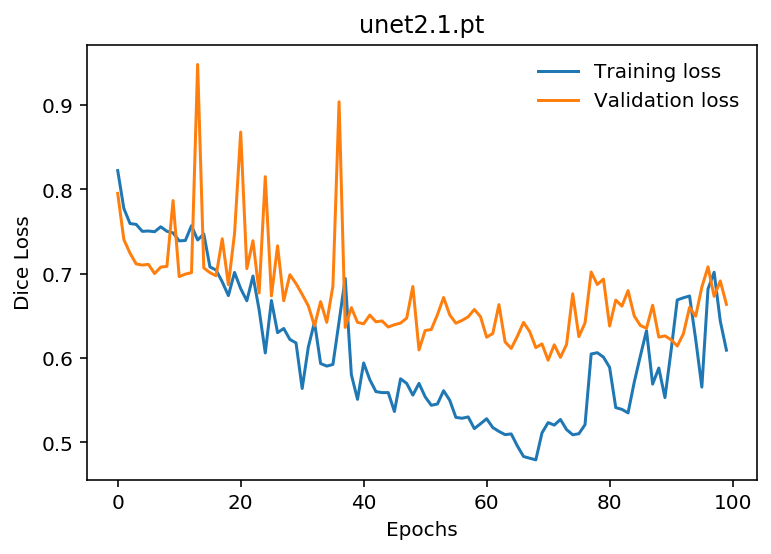
\includegraphics[scale=0.8]{img/unet2.1 100.png} 
\caption{Modelo miniunet2.1. 100 epochs. Se usa MiniUnet3D. Imagen objetivo con espaciado entre células. Sin data augmentation.}
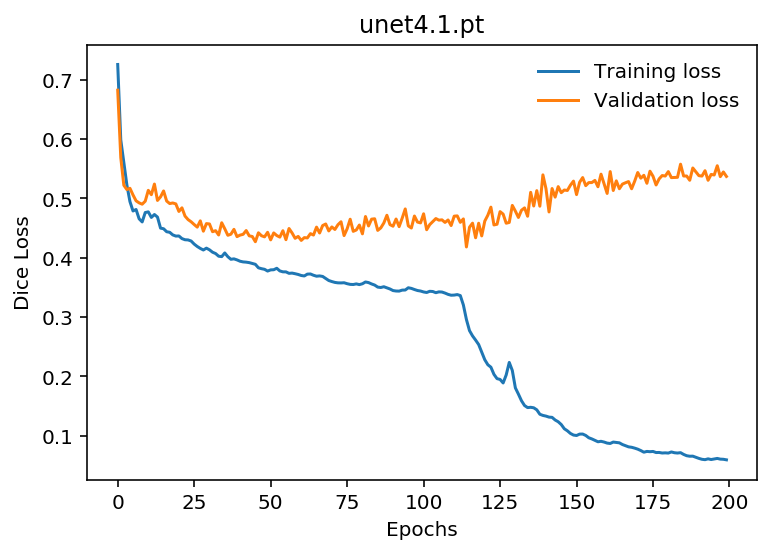
\includegraphics[scale=0.8]{img/unet4.1-200e-LQNOB-norm-Znorm.png} 
\caption{Modelo unet4.1. 200 epochs. Imagen objetivo con espaciado entre células. Sin data augmentation.}
\bigskip 
\end{figure}

\clearpage \subsubsection{Sin data augmentation vs Con data augmentation}
\begin{figure}[ht]
\centering
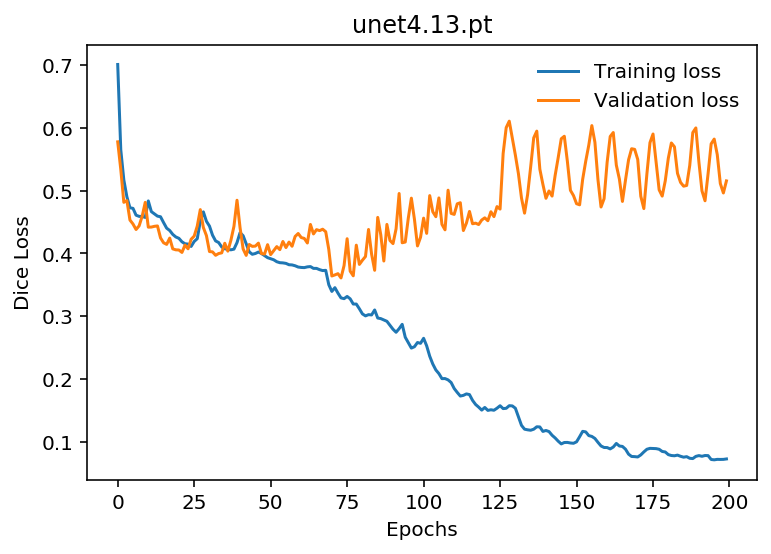
\includegraphics[scale=0.8]{img/unet4.13-200e-LQNOB-norm-Znorm.png} 
\caption{Modelo unet4.13. 200 epochs. Imagen objetivo con espaciado entre células. Sin data augmentation.}
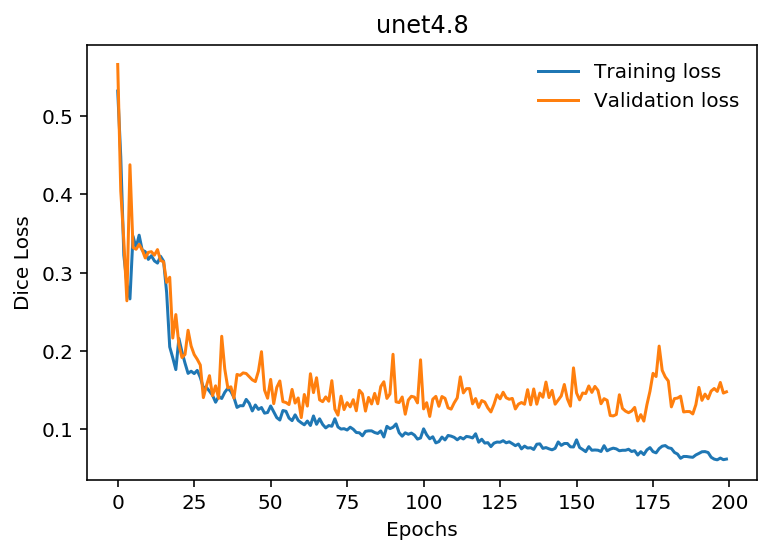
\includegraphics[scale=0.8]{img/unet4.8-200e-aug.png} 
\caption{Modelo unet4.8. 200 epochs. Imagen objetivo con espaciado entre células. Con data augmentation.}\bigskip 
\end{figure}

\clearpage \subsubsection{Sin Apex vs Con Apex}
\begin{figure}[ht]
\centering
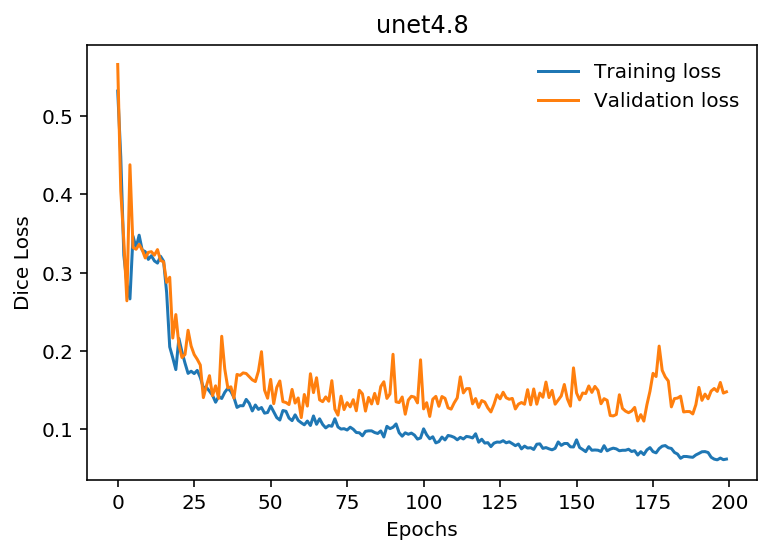
\includegraphics[scale=0.8]{img/unet4.8-200e-aug.png} 
\caption{Modelo unet4.8. 200 epochs. Imagen objetivo con espaciado entre células. Con data augmentation. Sin Apex}\bigskip 
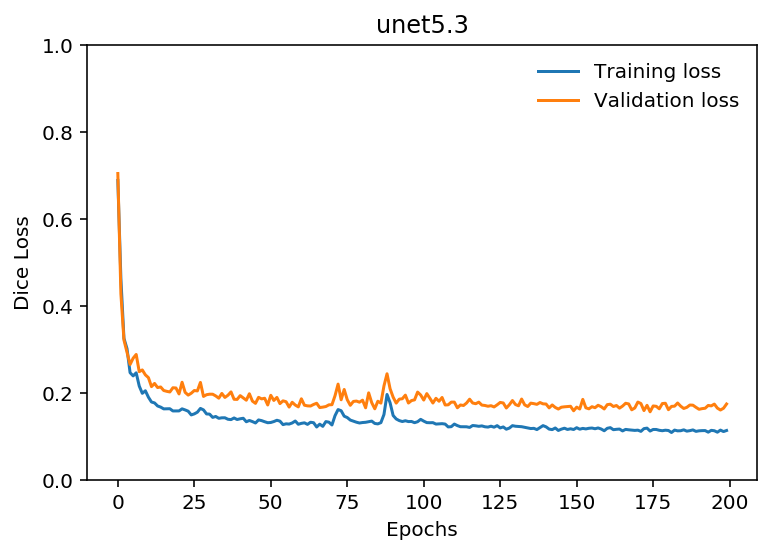
\includegraphics[scale=0.8]{img/unet5.2-sample-200e-target-apex.png} 
\caption{Modelo unet5.2. 200 epochs. Imagen objetivo con espaciado entre células. Con data augmentation. Con Apex.}\bigskip 
\end{figure}

\clearpage \subsubsection{Prueba de espaciado entre células.}
\begin{figure}[ht]
\centering
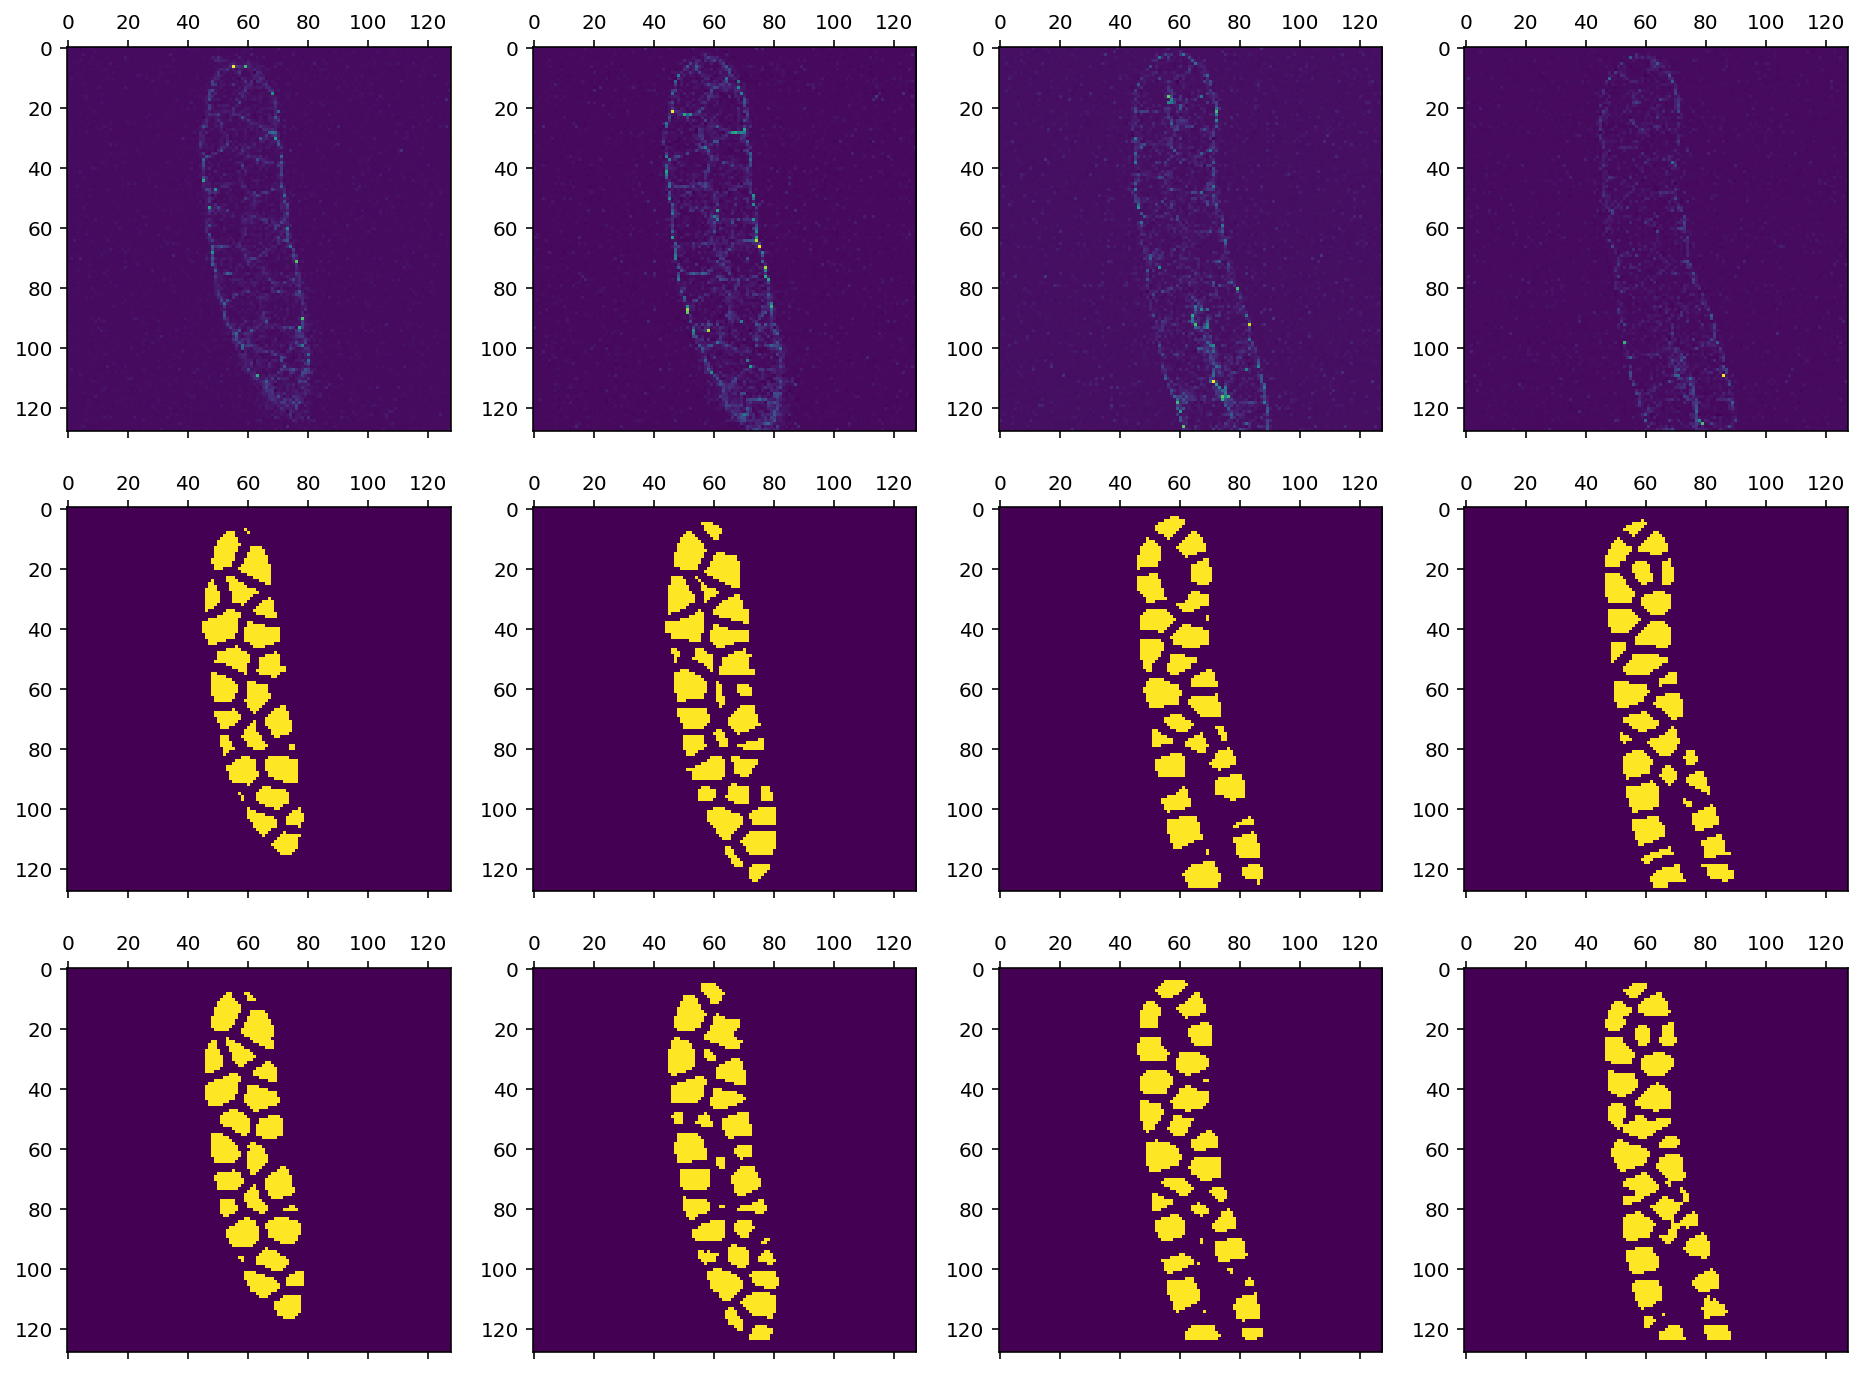
\includegraphics[scale=0.35]{img/unet6t-100e-resultados.png} 
\caption{Modelo unet6t. 100 epochs. Imagen objetivo con espaciado entre células. Con data augmentation. Pérdida Dice. Sin postprocesado. Primera fila imagen de entrada. Segunda fila segmentación objetivo. Tercera fila predicción. Z=20,25,45,50 en las columnas. IoU 0.72}\bigskip 
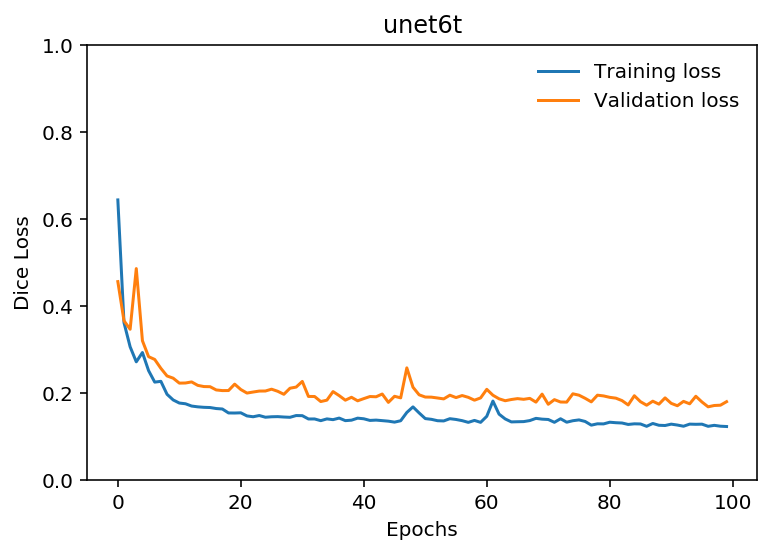
\includegraphics[scale=0.7]{img/unet6t.png} 
\caption{Modelo unet6t. 100 epochs. Imagen objetivo con espaciado entre células. Con data augmentation. Sin postprocesado.}\bigskip 
\end{figure}

\clearpage \subsubsection{Prueba de bordes.}
\begin{figure}[ht]
\centering
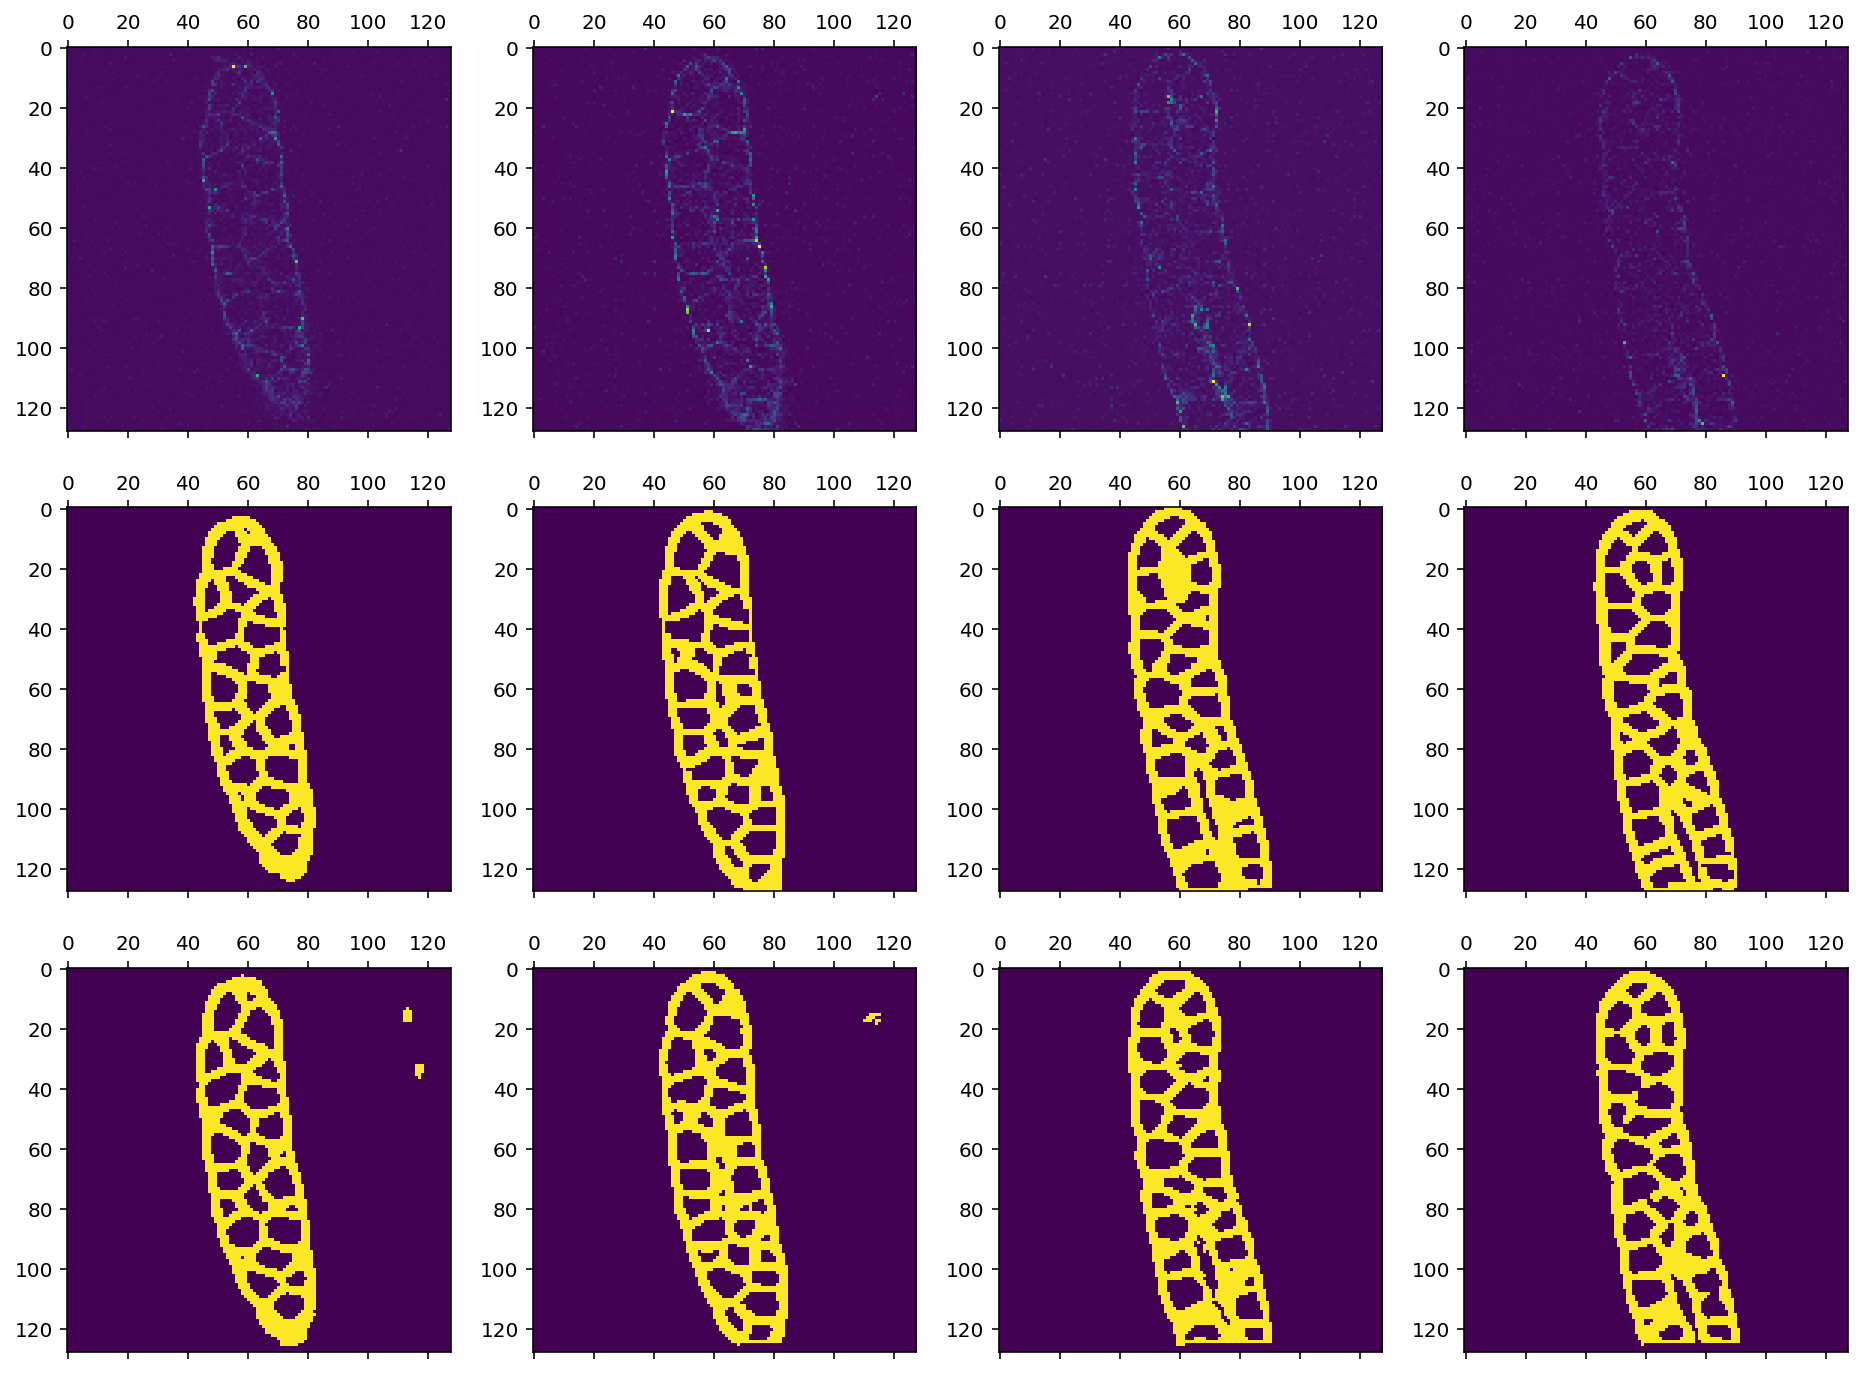
\includegraphics[scale=0.35]{img/unet6b-res.png} 
\caption{Modelo unet6b. 100 epochs. Imagen objetivo bordes de células. Con data augmentation. Pérdida Dice. Sin postprocesado. Primera fila imagen de entrada. Segunda fila segmentación objetivo. Tercera fila predicción. Z=20,25,45,50 en las columnas. IoU 0.84}\bigskip 
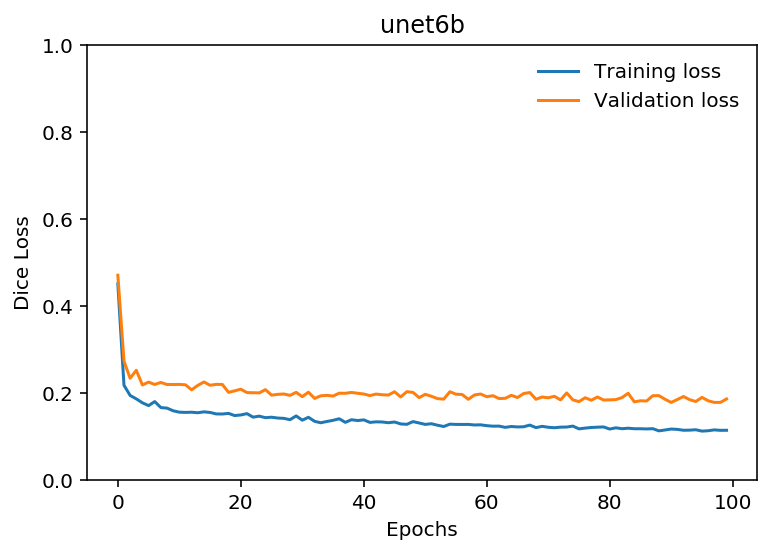
\includegraphics[scale=0.7]{img/unet6b-loss.png} 
\caption{Modelo unet6b. 100 epochs. Imagen objetivo bordes de células. Con data augmentation. Pérdida Dice. Sin postprocesado.}\bigskip 
\end{figure}

\clearpage \subsubsection{DT Watershed a bordes.}

\figura{1}{img/unet6b-color}{DT Watershed aplicado a la salida del modelo unet6b. Primera fila bordes. Segunda fila transformación de la distancia. Filtro gaussiano. Cuarta fila watershed con mínimos locales como semilla. Z=20,25,45,50 en las columnas.}{fig:unet6t-100e-resultados}{}

\clearpage \subsubsection{Comparación DT Watershed con espaciado entre células.}

\begin{figure}[ht]
\centering
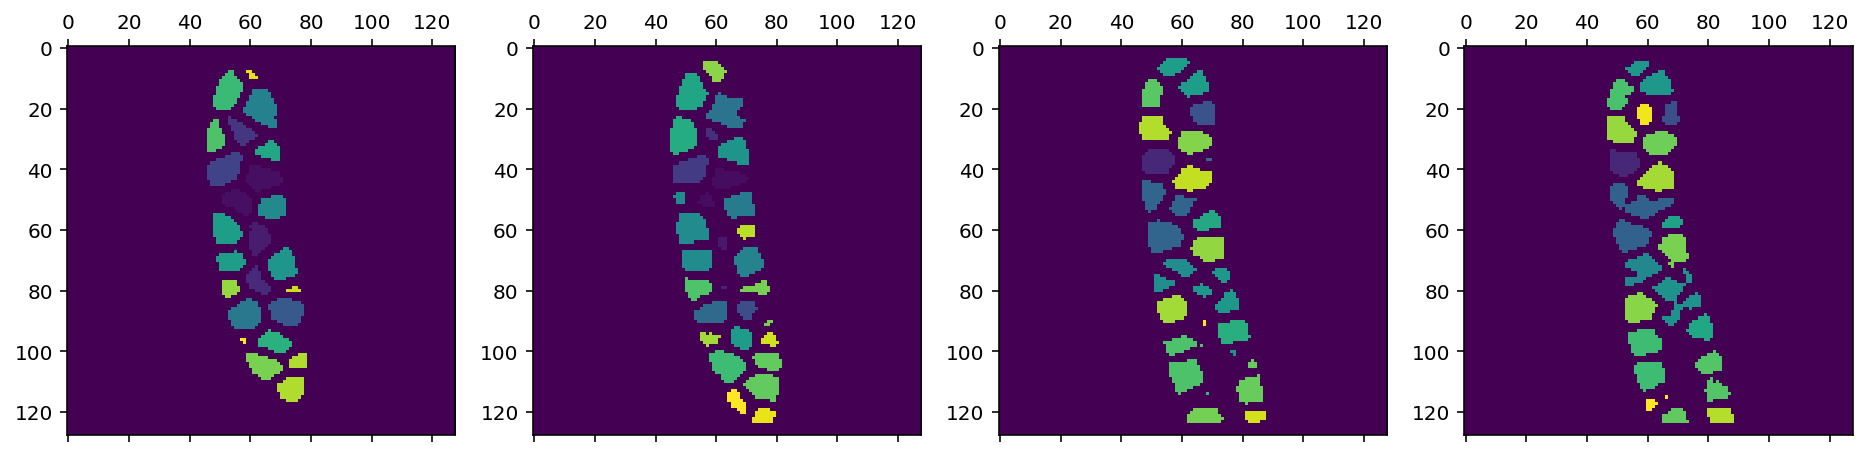
\includegraphics[scale=0.5]{img/unet6t-color.png} 
\caption{Modelo unet6b. 100 epochs. Imagen objetivo bordes de células. Con data augmentation. Pérdida Dice. Componentes conexas con etiquetas distintas. IoU 0.72}\bigskip 
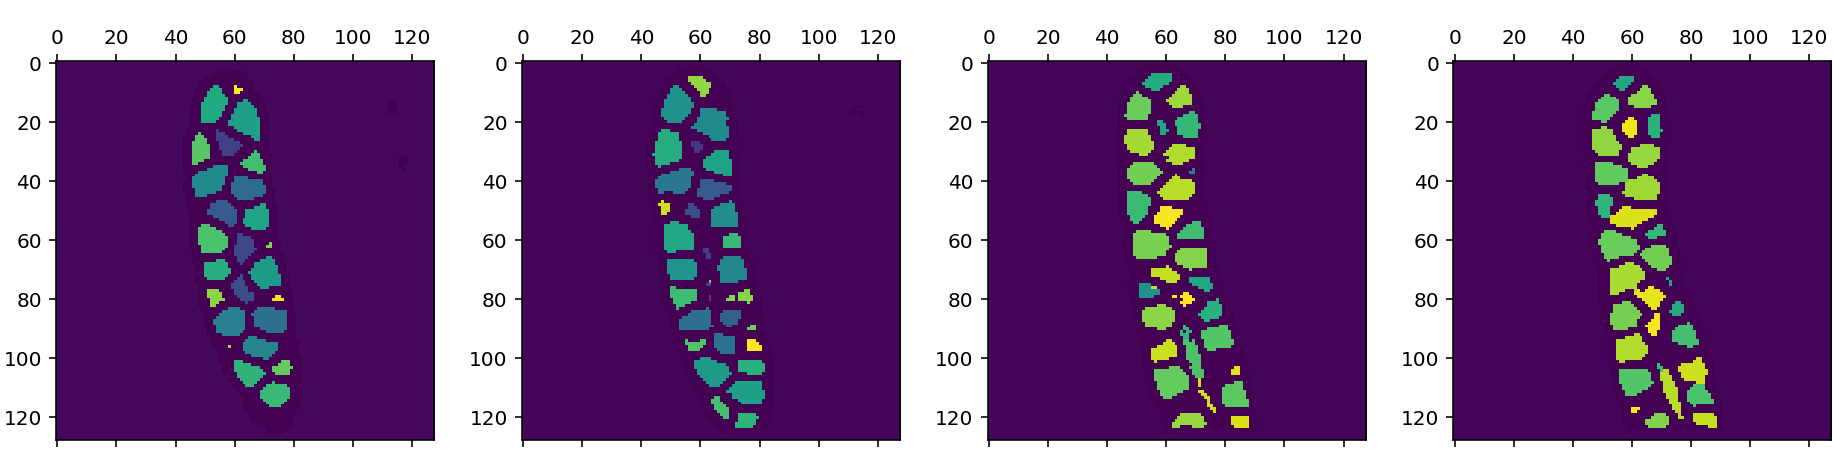
\includegraphics[scale=0.5]{img/unet6b-solocolor.png} 
\caption{DT Watershed aplicado a la salida del modelo unet6b. IoU 0.70}\bigskip 
\end{figure}
